\specialchapter{\texorpdfstring{PLATE IV. SYSTEMS OF TYPE \(D_{l}\) (\(l \geqslant 3\))}{PLATE IV. SYSTEMS OF TYPE D\_l (l >= 3)}}

\begin{enumerate}
\def\labelenumi{(\Roman{enumi})}
\tightlist
\item
  \(V = E = R^{l}\) . Roots: \(\pm\varepsilon_{i}\pm\varepsilon_{j}(1\leqslant i<j\leqslant l)\) ; ( \(\varepsilon_{i}\) ) the canonical basis of \(R^{l}\) . Number of roots: \(n = 2l(l - 1)\) .
\end{enumerate}

\begin{enumerate}
\def\labelenumi{(\Roman{enumi})}
\setcounter{enumi}{1}
\tightlist
\item
  Basis: \(\alpha_{1} = \varepsilon_{1} - \varepsilon_{2},\alpha_{2} = \varepsilon_{2} - \varepsilon_{3},\ldots ,\alpha_{l - 1} = \varepsilon_{l - 1} - \varepsilon_{l},\alpha_{l} = \varepsilon_{l - 1} + \varepsilon_{l}\) . Positive roots:
\end{enumerate}

\[
\varepsilon_ {i} - \varepsilon_ {j} = \sum_ {i <   k <   j} \alpha_ {k} (1 \leqslant i <   j \leqslant l).
\]

\[
\varepsilon_ {i} + \varepsilon_ {l} = \sum_ {i \leqslant k \leqslant l - 2} \alpha_ {k} + \alpha_ {l} (1 \leqslant i <   l),
\]

\[
\varepsilon_ {i} + \varepsilon_ {j} = \sum_ {i \leqslant k <   j} \alpha_ {k} + 2 \sum_ {j \leqslant k <   l - 1} \alpha_ {k} + \alpha_ {l - 1} + \alpha_ {l} (1 \leqslant i <   j <   l).
\]

\begin{enumerate}
\def\labelenumi{(\Roman{enumi})}
\setcounter{enumi}{2}
\item
  Coxeter number: \(h = 2l - 2\) .
\item
  Highest root:
\end{enumerate}

\[
\tilde {\alpha} = \varepsilon_ {1} + \varepsilon_ {2} = \alpha_ {1} + 2 \alpha_ {2} + \dots + 2 \alpha_ {l - 2} + \alpha_ {l - 1} + \alpha_ {l}.
\]

We have \(\tilde{\alpha} = \omega_2 + \omega_3\) if \(l = 3\) and \(\tilde{\alpha} = \omega_2\) if \(l \geqslant 4\) .

Completed Dynkin graph (l ≥ 4):

\pandocbounded{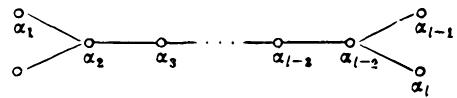
\includegraphics[keepaspectratio]{images/part002_b62b20f1.jpg}}

\begin{enumerate}
\def\labelenumi{(\Alph{enumi})}
\setcounter{enumi}{21}
\tightlist
\item
  \(R^{\prime} = R.\)
\end{enumerate}

\[
\Phi_ {R} (x, y) = \frac {(x | y)}{4 (l - 1)}, \quad \gamma (R) = 4 (l - 1) ^ {2}.
\]

\begin{enumerate}
\def\labelenumi{(\Roman{enumi})}
\setcounter{enumi}{5}
\tightlist
\item
  Fundamental weights:
\end{enumerate}

\[
\begin{array}{r l} \omega_ {i} & = \varepsilon_ {1} + \varepsilon_ {2} + \dots + \varepsilon_ {i} (1 \leqslant i \leqslant l - 2) \\ & = \alpha_ {1} + 2 \alpha_ {2} + \dots + (i - 1) \alpha_ {i - 1} + i (\alpha_ {i} + \alpha_ {i + 1} + \dots + \alpha_ {l - 2}) \\ & \quad + \frac {1}{2} i (\alpha_ {l - 1} + \alpha_ {l}) \\ \omega_ {l - 1} & = \frac {1}{2} (\varepsilon_ {1} + \varepsilon_ {2} + \dots + \varepsilon_ {l - 2} + \varepsilon_ {l - 1} - \varepsilon_ {l}) \\ & = \frac {1}{2} (\alpha_ {1} + 2 \alpha_ {2} + \dots + (l - 2) \alpha_ {l - 2} + \frac {1}{2} l \alpha_ {l - 1} + \frac {1}{2} (l - 2) \alpha_ {l}) \\ \omega_ {l} & = \frac {1}{2} (\varepsilon_ {1} + \varepsilon_ {2} + \dots + \varepsilon_ {l - 2} + \varepsilon_ {l - 1} + \varepsilon_ {l}) \\ & = \frac {1}{2} (\alpha_ {1} + 2 \alpha_ {2} + \dots + (l - 2) \alpha_ {l - 2} + \frac {1}{2} (l - 2) \alpha_ {l - 1} + \frac {1}{2} l \alpha_ {l}). \end{array}
\]

\begin{enumerate}
\def\labelenumi{(\Roman{enumi})}
\setcounter{enumi}{6}
\tightlist
\item
  Sum of the positive roots:
\end{enumerate}

\[
\begin{array}{r l} 2 \rho & = 2 (l - 1) \varepsilon_ {1} + 2 (l - 2) \varepsilon_ {2} + \dots + 2 \varepsilon_ {l - 1} \\ & = 2 (l - 1) \alpha_ {1} + 2 (2 l - 3) \alpha_ {2} + \dots + 2 (i l - \frac {i (i + 1)}{2}) \alpha_ {i} + \dots \\ & \qquad \dots + \frac {l (l - 1)}{2} (\alpha_ {l - 1} + \alpha_ {l}). \end{array}
\]

\begin{enumerate}
\def\labelenumi{(\Roman{enumi})}
\setcounter{enumi}{7}
\tightlist
\item
  Q(R): the set of points whose coordinates are integers with even sum.
\end{enumerate}

\[
\mathrm{P} (\mathrm{R}) = \bigoplus_ {i = 1} ^ {l} \mathbf {Z} \varepsilon_ {i} + \mathbf {Z} \left(\frac {1}{2} \sum_ {i = 1} ^ {l} \varepsilon_ {i}\right).
\]

l odd: \(\mathrm{P}(\mathrm{R})/\mathrm{Q}(\mathrm{R})\) is isomorphic to Z/4Z, generated by the image of \(\omega_{l}\) ; we have \(\omega_{1} \equiv 2\omega_{l}\) and \(\omega_{l-1} \equiv 3\omega_{l} \mod Q(\mathrm{R})\) . l even: \(\mathrm{P}(\mathrm{R})/\mathrm{Q}(\mathrm{R})\) is isomorphic to \((\mathbf{Z}/2\mathbf{Z}) \times (\mathbf{Z}/2\mathbf{Z})\) ; the three elements of order 2 are the images of \(\omega_{1}, \omega_{l-1}\) and \(\omega_{l}\) . Connection index: 4.

\begin{enumerate}
\def\labelenumi{(\Roman{enumi})}
\setcounter{enumi}{8}
\item
  Exponents: 1, 3, 5, \ldots, 2l - 5, 2l - 3, l - 1 (the last appearing twice if l is even and once if l is odd).
\item
  W(R) is the semi-direct product of the group \(S_{l}\) , acting by permutations of the \(\varepsilon_{i}\) , by the group \((\mathbf{Z}/2\mathbf{Z})^{l-1}\) , acting by \(\varepsilon_{i} \mapsto (\pm1)_{i}\varepsilon_{i}\) with \(\prod_{i}(\pm1)_{i} = 1\) . Its order is \(2^{l-1}.l!\)
\item
  \(l \neq 4\) : A(R)/W(R) = Z/2Z acting on the Dynkin graph by transposition of the nodes \(\alpha_{l-1}\) and \(\alpha_l\) . \(l = 4\) : A(R)/W(R) = \(\mathfrak{S}_3\) , acting on the Dynkin graph by permuting the nodes \(\alpha_1, \alpha_3\) and \(\alpha_4\) . \(w_0 = -1\) if \(l\) is even; \(w_0 = -\varepsilon\) if \(l\) is odd. where \(\varepsilon\) is the automorphism that interchanges \(\alpha_{l-1}\) and \(\alpha_l\) and leaves the other \(\alpha_i\) fixed.
\item
  Action of \(\mathrm{P}(\mathbb{R}^{-}) / \mathrm{Q}(\mathbb{R}^{-}) = \mathrm{P}(\mathbb{R}) / \mathrm{Q}(\mathbb{R})\) on the completed Dynkin graph: \(l\) odd: \(\omega_l\) transforms \(\alpha_0\) into \(\alpha_1\) , \(\alpha_l\) into \(\alpha_1\) , \(\alpha_1\) into \(\alpha_{l-1}\) and \(\alpha_{l-1}\) into \(\alpha_0\) ; it interchanges \(\alpha_j\) and \(\alpha_{l-j}\) for \(2 \leqslant j \leqslant l - 2\) . \(l\) even: \(\omega_l\) (resp. \(\omega_{l-1}\) ) interchanges \(\alpha_0\) and \(\alpha_l\) (resp. \(\alpha_0\) and \(\alpha_{l-1}\) ), \(\alpha_1\) and \(\alpha_{l-1}\) (resp. \(\alpha_1\) and \(\alpha_l\) ) and interchanges \(\alpha_j\) and \(\alpha_{l-j}\) for \(2 \leqslant j \leqslant l - 2\) .
\end{enumerate}

\[
\left( \begin{array}{c c c c c c c} 2 & - 1 & \dots & 0 & 0 & 0 & 0 \\ - 1 & 2 & \dots & 0 & 0 & 0 & 0 \\ \vdots & \vdots & \ddots & \vdots & \vdots & \vdots & \vdots \\ 0 & 0 & \dots & 2 & - 1 & 0 & 0 \\ 0 & 0 & \dots & - 1 & 2 & - 1 & - 1 \\ 0 & 0 & \dots & 0 & - 1 & 2 & 0 \\ 0 & 0 & \dots & 0 & - 1 & 0 & 2 \end{array} \right)
\]

\begin{enumerate}
\def\labelenumi{(\Roman{enumi})}
\setcounter{enumi}{12}
\tightlist
\item
  Cartan matrix \((l\times l)\) :
\end{enumerate}

